% Fly-by-Wire v2 (2026-10-01 KST, 구 명칭 대체): 옛 paper/를 버리고 뼈대(D:/tools/scratch_qdd/board/PAPER_SKELETON.md) 기준으로 새로 쓴 초안.
% 중심: (1) 로봇을 조종하는 상위 VLM, (2) 좁은 조이스틱 JCR(Joystick-Conditioned Reflex)와 성능 손실 없이 잇는 결합 방법.
% 규칙(NOW.md §4): Astra·교사 정책 없음(시뮬 라벨 = 시뮬 참값(특권 정보로 계산)), 3인칭 영상 없음, 확정 전 수치는 \tentative(주황).
% 서식·글꼴은 옛 paper/main.tex·preamble.tex(CVPR author kit + 나눔고딕) 그대로. 빌드: tectonic -X compile main.tex
% 그림: figures/src/make_figs_v2.py (F1-F8), evidence·eval_protocol은 paper/figures/src/make_figs_pn.py 산출물을 복사.

\documentclass[10pt,twocolumn,letterpaper]{article}
\usepackage[review]{cvpr}
%% This file contains a number of tweaks that are typically applied to the main document.
%% They are not enabled by default, but can be enabled by uncommenting the relevant lines.


%%
%% Official support for 2-column teaser figure
%%
\usepackage{cuted} %< for strip environment

%%
%% For auto-referencing of figures (see fig/teaser.tex and \label{} therein) 
%%
\usepackage{currfile} %< for \currfilebase macro

%%
%% caption and (global) spacing overrides
%%
\usepackage{caption} %< for "\captionof" commands (teaser)
% \setlength{\abovecaptionskip}{.5em} % space above caption
% \setlength{\belowcaptionskip}{1em} % space below caption

%%
%% Inline annotations; for predefined colors, refer to "dvipsnames" in the xcolor package:
%% https://tinyurl.com/overleaf-colors
%%
\newcommand{\red}[1]{{\color{red}#1}}
\newcommand{\todo}[1]{{\color{red}#1}}
\newcommand{\TODO}[1]{\textbf{\color{red}[TODO: #1]}}
%%
%% Disable for camera ready / submission by uncommenting these lines:
%%
% \renewcommand{\TODO}[1]{}
% \renewcommand{\todo}[1]{#1}

%%
%% Work harder in optimizing text layout. Typically shrinks text by 1/6 of page, enable
%% it at the very end of the writing process, when you are just above the page limit.
%%
% \usepackage{microtype}

%%
%% Fine-tune paragraph spacing.
%%
% \renewcommand{\paragraph}[1]{\vspace{.5em}\noindent\textbf{#1.}}

%%
%% Globally adjusts space between figure and caption.
%%
% \setlength{\abovecaptionskip}{.5em}

%%
%% Allows "the use of \paper to refer to the project name"
%% with automatic management of space at the end of the word.
%%
% \usepackage{xspace}
% \newcommand{\paper}{ProjectName\xspace}

%%
%% Commonly used math definitions.
%%
% \DeclareMathOperator*{\argmin}{arg\,min}
% \DeclareMathOperator*{\argmax}{arg\,max}

%%
%% Tighten underline.
%%
% \usepackage{soul}
% \setuldepth{foobar}

%%
%% Reconfigure paragraph (tweaks spacing)
%%

%%
%% [Harvest] 한국어(XeLaTeX)와 마인드맵 표시
%%
\usepackage{kotex}
% 한글 글꼴: 나눔고딕(OFL, fonts/ 폴더에 동봉 — 로컬과 Overleaf에서 같은 결과). 기본 은바탕보다 화면 가독성이 좋다(사용자 요청 2026-09-24). 한글은 기울이지 않는다(기울임 자리도 바로 선 글꼴).
\setmainhangulfont{NanumGothic}[Path=fonts/, Extension=.ttf, UprightFont=*-Regular, BoldFont=*-Bold, ItalicFont=*-Regular, BoldItalicFont=*-Bold]
\setsanshangulfont{NanumGothic}[Path=fonts/, Extension=.ttf, UprightFont=*-Regular, BoldFont=*-Bold, ItalicFont=*-Regular, BoldItalicFont=*-Bold]
\usepackage{enumitem}
\setlist{nosep,leftmargin=1.2em}
\newcommand{\intent}[1]{\textcolor{red}{#1}}      % 빨간색 = 사용자가 의도하고 말한 것
\newcommand{\idea}[1]{\textbf{지금 생각:} #1}
\newcommand{\chg}[1]{\textbf{바뀐 점:} #1}
\newcommand{\dirn}[1]{\textbf{방향:} #1}
\newcommand{\decide}[1]{\textbf{[결정 필요]} #1}
%% [Harvest] 논문 판(2026-09-25, user-log 63): 아직 확실하지 않은 수치·주장은 주황색으로 둔다.
\definecolor{tentorange}{RGB}{226,112,0}
\newcommand{\tentative}[1]{\textcolor{tentorange}{#1}}   % 임시: 계획값, 가정값, 파이프라인 시험 값
\newcommand{\todoexp}[1][---]{\textcolor{tentorange}{#1}} % 결과 예정 칸(표의 빈 칸)
\usepackage{multirow}
\usepackage{makecell}

\definecolor{cvprblue}{rgb}{0.21,0.49,0.74}
\usepackage[pagebackref,breaklinks,colorlinks,allcolors=cvprblue]{hyperref}

\def\paperID{*****}
\def\confName{CVPR}
\def\confYear{2026}

\title{Fly-by-Wire Manipulation: A Large VLM Pilots the Robot,\\a Joystick-Conditioned Reflex Keeps It in the Envelope\\ --- 상위 VLM이 직접 조종하고 조이스틱 JCR는 허용 범위 안에서만 지키는 로봇 조작}

\author{익명 저자\\
익명 기관}

\begin{document}
\maketitle
\begin{abstract}
지금의 VLA는 3--8B VLM 하나가 계획·판단·명령·움직임을 모두 떠안는다. 그 크기의 모델에게는 무거운 짐이고, VLM에서 행동 전문가로 넘어가며 정보도 잃는다. Fly-by-Wire는 이 짐을 나눈다. 학습 가능한 크기의 상위 VLM(Qwen3.5-35B-A3B, LoRA)이 계획·판단·명령을 모두 맡고, 머리 영상 위의 점과 높이 의도로 로봇을 조종한다. 목표 좌표는 모델이 아니라 코드가 센서 깊이로 계산한다. 상위는 결합을 위해 다시 학습하지 않는다: 규칙 코드 어댑터(학습 없음)가 상위 출력(점·높이 의도·그리퍼 의도·평가)을 목적지 xyz, 대상 물체 마스크, 단계, 그리퍼 허용, 단계별 끌림 세기(운반 중 약, 잡기·놓기 근처 강 — 딱딱한 범위 대신 목적지로 당김, 넓은 안전 범위만 자름)로 바꾼다. 하위 JCR(Joystick-Conditioned Reflex, 조이스틱 반사 정책: 언어·계획 없이 그 끌림을 따르고, 잡기·놓기 시점과 접촉만 판단하는 반사 정책)는 이 끌림을 좇는 좁은 조이스틱이며, 이상 신호는 어댑터가 문장으로 바꿔 상위의 다음 호출에 실어 보낸다. 두 모듈이 각자 최대 성능을 내도 연결에서 성능이 샐 수 있으므로, 우리는 연결 손실을 같은 시드의 2$\times$2 참값 교체(어댑터 포함)로 정의하고 5\,\%p 이하를 합격 기준으로 둔다. 재질의는 도착 뒤(상위가 학습한 장면 그대로)이며, 상위가 1--3\,s 생각하는 동안 JCR가 정렬·잡기·들기 시작을 이어가 로봇이 멈추지 않는다. 상위는 동결하고, JCR만 어댑터가 실제로 내는 명령(상위 흉내 명령도 어댑터 통과) 위에서 학습해 맞물린다. 지금까지 사전 등록 실험에서 깊이 점 출력은 본 적 없는 탁자 높이에서 \tentative{3.5\,mm}를 유지했고(거리 숫자 출력은 \tentative{31--71\,mm}), 공개 로봇 데이터의 점 라벨은 새 물체 오차를 \tentative{85.3}에서 \tentative{4.0\,mm}로 줄였다. 시뮬 참값 명령을 스크립트 실행기가 따르면 \tentative{40/40}이었지만 기존 VLA를 조이스틱으로 쓰면 \tentative{1/40}이었다. 폐루프 상태 분포와 근접 미세 조종을 배우지 않은 탓이며, 그래서 JCR는 자기 롤아웃에 시뮬 참값을 다시 붙여 반복 학습한다.
\end{abstract}

\section{문제와 동기}
\label{sec:problem}

\paragraph{한 모델이 모든 짐을 진다.} 기존 VLA는 안의 VLM(3--8B)이 과제 계획, 진행 판단, 다음 명령, 실제 움직임을 전부 맡는다. 이 크기의 VLM에게는 너무 무거운 짐이다. 게다가 판단은 VLM의 언어·시각 표현에서 이루어지고 움직임은 행동 전문가가 만들기 때문에, 그 사이의 전이에서 정보가 손실된다.

\paragraph{큰 VLM은 판단은 잘하지만 느리다.} 판단을 큰 VLM에게 맡기면 정확도는 오르지만 한 번 답하는 데 초 단위가 걸린다. 큰 VLM 혼자 제어하면 명령과 명령 사이에 로봇이 새 정보를 보지 못하는 `장님 구간'이 생기고, 1단계 구현에서는 로봇이 답을 기다리며 멈춘다(\cref{fig:timeline}a).

\paragraph{목표.} 큰 VLM의 판단력과 작은 JCR의 빠른 반응을 \emph{성능 손실 없이} 잇는다. 이를 위해 (i) 계획·판단·명령은 상위 VLM에 모으고, (ii) JCR에게는 상위 명령 기준의 미세 조종이라는 단순한 일만 주며, (iii) 두 모듈을 잇는 과정에서 새는 성능을 직접 재고 줄인다. 따라서 JCR의 설계·학습·평가는 JCR가 스스로 계획하는 쪽으로 가지 않는다. JCR 입력의 목표는 상위 명령이고, 출력은 허용 범위 안의 보정과 이상 신호뿐이다.

\section{핵심 가설}
\label{sec:hyp}

\begin{itemize}
  \item \textbf{H-J (짐 덜기).} 계획·판단·명령을 상위 VLM이 모두 맡고 VLA는 조이스틱(명령 기준 미세 조종)만 하면, 같은 VLA가 혼자 할 때보다 낫다. 검증은 같은 VLA를 단독 모드(스스로 계획)와 조이스틱 모드로 같은 과제·시드에서 돌려 비교한다(\cref{sec:eval}). 단독 모드는 비교용으로만 둔다.
  \item \textbf{H-L (학습 가능한 상위).} 학습 가능한 크기(35B-A3B, LoRA)의 VLM을 시뮬 참값(특권 정보로 계산)과 공개 로봇 데이터의 점 라벨로 특화하면, 로봇을 조종하는 상위로 쓸 만하다.
  \item \textbf{H-C (연결 손실).} 잘 설계한 연결은 두 모듈의 성능을 거의 깎지 않는다. 연결 손실(\cref{sec:closs}) $\le$ 5\,\%p, 연결 탓 실패 $\le$ 전체 실패의 10\,\%를 합격 기준으로 둔다.
\end{itemize}
H-L은 지금 근거가 가장 많고(\cref{sec:evidence}), H-J와 H-C는 결합 실험(\cref{sec:coupling})이 직접 겨누는 가설이다.

\section{전체 구조: Fly-by-Wire}
\label{sec:structure}

\begin{figure*}[t]
\centering
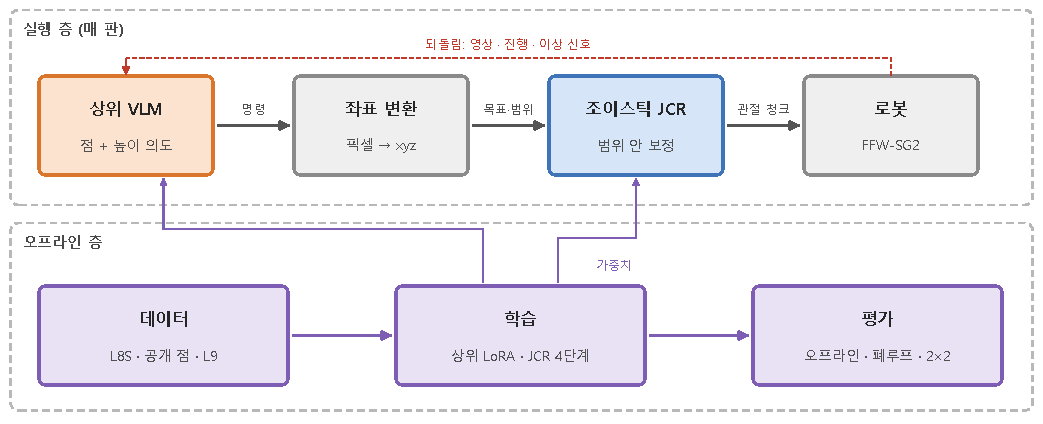
\includegraphics[width=\linewidth]{figures/f1_overview.pdf}
\caption{\textbf{전체 파이프라인.} 위: 실행 층. 상위 VLM이 머리 영상 위의 점과 높이 의도를 내면(재학습 없이 지금 학습한 형식 그대로), 코드 어댑터가 깊이로 xyz를 계산해 대상 마스크·단계·그리퍼 허용·단계별 끌림 세기로 바꿔 조이스틱 JCR에 준다. JCR는 그 끌림을 따라 보정해 로봇에 관절 청크를 보낸다. JCR 보고(접촉·잡기 성공·이상 신호)는 어댑터가 문장으로 바꿔 상위의 `직전 명령과 결과' 입력 칸에 넣는다. 아래: 오프라인 층. 데이터(L8S·공개 점·L9)로 JCR를 학습하고(상위는 동결), 오프라인 점·폐루프·결합 2$\times$2로 평가한다. 세부는 \cref{fig:upper,fig:vla,fig:timeline,fig:train,fig:closs,fig:data}.}
\label{fig:overview}
\end{figure*}

조종사는 조이스틱으로 직접 조종하며 권한을 전부 갖고, 비행 제어 컴퓨터는 조종사가 정한 목적지로 끌어당기며 안정화·보정할 뿐 목적지를 정하지 않고 넓은 안전 범위만 지킨다. Fly-by-Wire에서 조종사는 상위 VLM, 조종간 신호를 비행 제어 컴퓨터가 쓰는 신호로 바꾸는 장치는 코드 어댑터, 비행 제어 컴퓨터는 JCR다(\cref{fig:overview}).

\paragraph{권한.} 명령 권한은 항상 상위에 있다. 목표, 높이 의도, 그리퍼 의도, 진행 평가와 검증은 상위가 낸다. 코드 어댑터(규칙, 학습 없음)가 이를 JCR 명령으로 바꿀 뿐 새 목표를 만들지 않는다. JCR는 어댑터가 정한 끌림을 따라 움직임을 고치고, 이상 신호를 내어 상위를 일찍 다시 부를 근거를 준다. JCR는 과제를 고르거나 상위 목표를 바꾸지 않는다.

\paragraph{한 판의 흐름.} 상위가 목표를 낸다 $\rightarrow$ 어댑터가 명령으로 바꾼다 $\rightarrow$ 실행(1단계는 결정적 실행기, 2단계는 JCR) $\rightarrow$ 도착 뒤 상위에게 다시 묻는다(상위가 학습한 장면 그대로); 상위가 생각하는 1--3\,s 동안 JCR는 정렬·잡기·들기 시작을 이어가 로봇이 멈추지 않는다 $\rightarrow$ 검증 $\rightarrow$ 반복. 잡음·놓음의 확정은 그리퍼 폭·전류를 보는 고유 감각 코드(T1)가 맡고, 상위는 결과를 보고 다음 단계를 고른다.

\paragraph{두 단계로 검증한다.} 1단계는 상위 단독이다. 상위 명령을 결정적 실행기가 평균 약 8\,cm/s의 최소 저크 직선 운동으로 수행하고, 로봇은 상위의 답을 기다린다. 실행기에는 재학습 없는 두 규칙이 있다. 쥐기 전에 깊이로 잰 대상 점을 기억해 두었다가 든 물체가 놓을 곳을 가릴 때 쓰고, `위' 의도가 같은 목표에서 되풀이되면 다음 단계로 넘긴다. 2단계는 실행기 자리에 코드 어댑터 + 조이스틱 JCR를 넣어, 상위가 생각하는 동안 JCR가 이어가며 기다림을 없앤다(\cref{sec:coupling}). 1단계는 결합의 비교 기준으로 남는다.

\paragraph{플랫폼.} 기준 로봇은 ROBOTIS AI Worker FFW-SG2다(7자유도 팔 두 개, 평행 그리퍼, 2자유도 머리, 리프트, 팔마다 100\,Hz 위치 명령). 카메라는 기본 장착분만 쓴다. 머리 ZED Mini 672$\times$376, 손목 RealSense D405 두 대다. 머리는 45$^\circ$가 기본이다. 안전 규칙으로 팔 관절 한 걸음은 0.04\,rad 이하로 묶는다. 시뮬은 Isaac Sim 5.1과 Isaac Lab 2.3이다.

\section{상위 VLM 조종기}
\label{sec:upper}

\begin{figure*}[t]
\centering
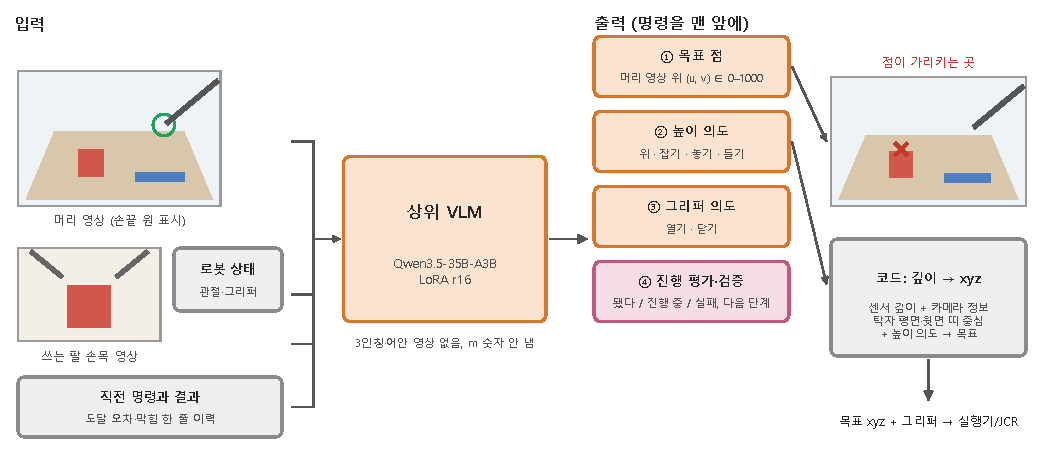
\includegraphics[width=\linewidth]{figures/f2_upper_call.pdf}
\caption{\textbf{상위 VLM 조종 한 호출.} 입력은 손끝 원만 그린 머리 영상, 표시 없는 쓰는 팔 손목 영상, 로봇 상태, 직전 명령과 결과다. 출력은 머리 영상 위 목표 점, 높이 의도, 그리퍼 의도, 진행 평가·검증이며 명령 부분을 답의 맨 앞에 둔다. 모델은 m 숫자를 말하지 않는다. 점이 가리키는 곳의 xyz는 코드가 센서 깊이와 카메라 정보로 계산한다.}
\label{fig:upper}
\end{figure*}

\subsection{입력과 출력}
\paragraph{입력.} 머리 영상(손끝 위치를 알리는 원만 그림)과 지금 쓰는 팔의 손목 영상(아무것도 그리지 않음), 로봇 자기 상태(관절, 그리퍼 폭), 직전 명령과 그 결과(도달 오차·막힘을 적은 한 줄 이력)다(\cref{fig:upper}). 3인칭·어안 영상은 정확도 위험이 있어 쓰지 않는다. 영상에 격자는 그리지 않는다. 로봇 자기 정보(좌표계, 그리퍼 형상, 카메라 자세·내부값)는 URDF·관절 상태·camera\_info에서 코드가 만든다.

\paragraph{출력: 줄기 D.} 모델은 (i) 머리 영상 위의 목표 점(0--1000 정규화), (ii) 높이 의도(위, 잡기, 놓기, 들기), (iii) 그리퍼 의도, (iv) 진행 평가·검증을 낸다. 목표 xyz는 코드가 계산한다. 센서 깊이와 카메라 정보로 탁자 평면을 맞추고, 평면 위 물체 영역의 윗면 띠 중심을 잡은 뒤 높이 의도에 맞춰 목표를 정한다. 실물에서는 머리 스테레오와 손목 D405의 깊이가 필요하며, 이는 사람이 준 정보가 아니라 측정값이다.

\subsection{왜 D인가}
거리를 m 숫자로 직접 내는 줄기는 본 적 없는 탁자 높이에서 무너졌다. 한 높이 데이터로 학습한 8B와 35B 모두 새 높이 3D 오차가 \tentative{약 31\,mm}였고, 대부분 z 오차였다. 모델 크기로 풀리지 않는다. 같은 편을 출력 형식만 바꿔 비교하자 깊이 점만 새 높이에서 \tentative{3.5--3.6\,mm}를 유지했다(깊이 없는 xyz \tentative{31--71\,mm}, 폐루프 \tentative{8/8}). 깊이가 있으면 쓰고 없으면 xyz를 직접 내는 하이브리드 H와의 비교에서도 D가 새 물체에서 \tentative{4.0} 대 \tentative{83.7\,mm}로 이겼다(\cref{sec:evidence}).

사람이 준 손 정보(탁자 높이 등)는 넣지 않는다. 참 탁자 높이를 입력으로 받은 판만 새 높이에 맞았고(\tentative{4.0\,mm}), 학습 때만 그 정보를 쓰는 세 방법은 \tentative{10.9--20.5\,mm}였다. 영상 하나로는 탁자 높이를 약 2\,cm보다 정확히 알 수 없고, 실제 환경에는 참값이 없다. 척도와 높이는 깊이가 맡는다.

\subsection{판단의 역할}
상위는 명령만 내지 않고 매 답에 판단을 싣는다.
\begin{itemize}
  \item \textbf{진행 평가:} 끝낸 일·지금 하는 일·남은 일과 현재 단계의 상태(됐다 / 진행 중 / 실패).
  \item \textbf{실패 감지와 다시 계획:} 직전 명령의 결과(측정 이력, VLA 이상 신호, 새 영상)가 의도와 어긋나면 실패로 판정하고 목표를 다시 낸다.
  \item \textbf{다음 단계 선택:} 결과를 확인한 뒤 잡기·나르기·놓기 가운데 다음을 고른다. 쥠·놓음의 확정 근거는 T1이다.
\end{itemize}
판단 정확도(진행 판정의 정밀도·재현율, 실패 감지까지의 지연)를 재는 평가 세트는 아직 없다. 이 지표는 \cref{sec:questions}의 첫 질문이다. 실패 인지·재시도를 위한 회복 데이터도 이번 본 학습에는 넣지 않았다.

\subsection{학습}
\label{sec:upper_train}
라벨은 시뮬 참값(특권 정보로 계산)이다. 로봇 기하와 시뮬 상태에서 도출한 규칙이 같은 요청에 대해 낸 답을 정답으로 쓴다. 공개 로봇 데이터는 행동 라벨이 아니라 머리 시점 영상 위의 점 라벨(대상, 놓을 곳, 그리퍼)로만 쓴다~\cite{molmoact2026}. 공개/시뮬 비율은 $\min(0.75,\ 2\times\text{공개 풀}/\text{시뮬 행})$이고 같은 행의 반복은 2배까지다.

\paragraph{본 35B.} Qwen3.5-35B-A3B에 LoRA(r16, $\alpha$32, 어텐션·DeltaNet·공유 전문가), lr $10^{-4}$, H200 4장 전역 배치 24로 3 에폭(약 25,300걸음) 학습한다. 데이터는 202,397행이다(L8S 139,603행 + 공개 점 62,794행, \cref{sec:data}). 2026-09-30 15:57 KST에 시작했고 \tentative{10/1 오후} 끝날 예정이다. 최적 에폭은 학습에 쓰지 않은 L8S 보류 검증 분할(편 단위 3\,\%)의 20\,mm 초과 실패율로 고르며, OOD·새 물체 세트로는 고르지 않는다. 이 규칙은 결과 전에 사전 등록했다.

\paragraph{다음.} 도착 전에 다음 명령을 내는 행(\cref{sec:mesh})과 L9 데이터(\cref{sec:data})를 넣은 다음 본 학습은 기본 모델부터 섞어 한 번에 학습한다.

\section{하위 조이스틱 JCR}
\label{sec:vla}

\begin{figure*}[t]
\centering
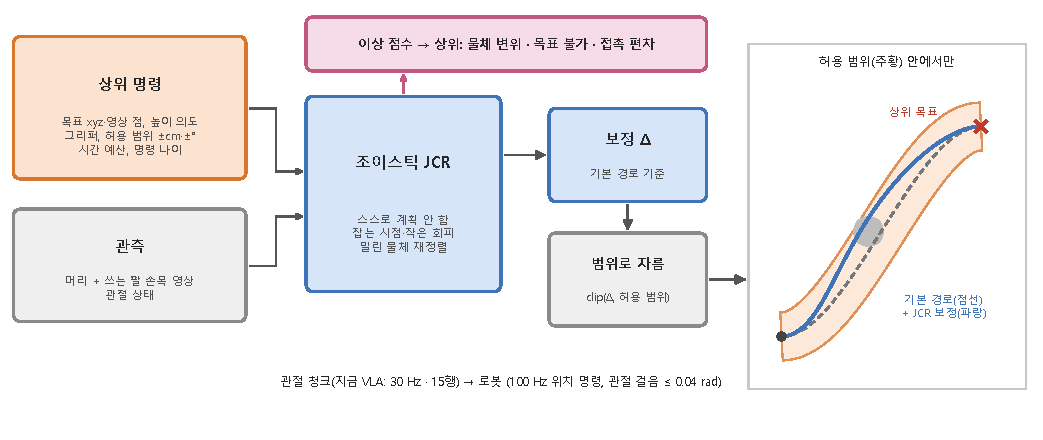
\includegraphics[width=\linewidth]{figures/f3_vla.pdf}
\caption{\textbf{조이스틱 JCR.} 상위 명령(목표·의도·그리퍼·허용 범위·명령 나이)과 관측을 받아, 명령이 만든 기본 경로에 대한 보정을 TCP 변위 청크로 내고 허용 범위로 자른다. 오른쪽: 기본 경로(점선)와 JCR 보정(파랑)은 허용 범위(주황) 밖으로 나가지 않는다. 이상 신호는 상위를 일찍 다시 부르는 근거가 된다.}
\label{fig:vla}
\end{figure*}

\paragraph{역할.} JCR(Joystick-Conditioned Reflex, 조이스틱 반사 정책)는 세 가지만 맡는다. (i) 조이스틱 따라가기, 곧 상위 명령 기준의 미세 조종, (ii) 잡기·놓기 시점, (iii) 접촉 여부 판단이다. 계획·단계 선택·목표 결정은 하지 않고 언어 명령도 받지 않는다(\cref{fig:vla}). 설계·데이터·학습·평가는 모두 상위가 명령을 준다는 전제 위에 있다. 시뮬 참값 명령은 상한을 재는 데만 쓴다.

\paragraph{입력.} 머리·쓰는 팔 손목 영상과 고정된 짧은 문장(단계 문장 없음), 그리고 조건 네 가지다. 조이스틱 $j$는 상위 목표 $-$ 손끝이며, 몸통 고정 좌표계의 연속 3D 값으로 양자화나 사각지대가 없다. 허용 범위는 목표 구 반경, 경로 관 반경, 허용 그리퍼 방향이다. 명령 나이는 명령이 나온 뒤 지난 시간이다. 고유 감각은 관절, 그리퍼 폭·전류(effort), 인과 후방 차분 속도, 현재 명령 관절이다. 단계 문장을 빼는 이유는 그리퍼 시점이 접촉이 아니라 문장에 붙기 때문이다(\cref{sec:evidence}).

\paragraph{출력과 권한.} 팔 행동은 현재 명령 TCP 기준의 변위 청크다(20\,Hz, 10행 = 0.5\,s, 0.2\,s마다 새 청크). 손끝 방향과 IK(중력 처짐 보정, 관절 한 걸음 0.04\,rad 이하)는 코드가 맡는다. 그리퍼는 행마다 \{유지, 닫기, 열기\} 사건을 내고, 접촉 확률 두 개(패드--대상, 예상 밖 접촉)를 낸다. 이상 신호는 별도 이진 머리(예상 밖 접촉, 대상 이동, 떨어짐, 명령 불일치, 복구 불가)와 멈춤 출력이며, 문턱은 보류 세트에서 등각(conformal) 방식으로 오탐률 5\,\%에 맞춘다~\cite{faildetect2025}. 실행되는 움직임은
\begin{equation}
  a_t = a^{\text{nom}}_t + \mathrm{clip}\bigl(\Delta_t,\ \mathcal{E}(c)\bigr),
\end{equation}
이며 $a^{\text{nom}}$은 명령 $c$가 만든 기본 경로, $\mathcal{E}(c)$는 명령이 허용한 범위다. 자름과 허용 그리퍼 방향은 코드가 강제하므로 JCR가 틀려도 상위 명령에서 범위 이상 벗어나지 않는다. 바탕 모델은 Qwen3-VL-4B~\cite{qwen3vl2025} LoRA 백본과 흐름 정합 행동 전문가이며, 전문가에서 백본으로 가는 기울기는 막는다~\cite{kinsulate2025}.

\paragraph{정답: 허용 범위에 투영한 시뮬 참값.} 참값 목표 $c^\ast$는 특권 물체 자세로 계산한 실제 잡기·놓기 자세를 허용 범위(목표 구 $\cup$ 경로 관)에 투영한 점이다. 명령이 조금 틀렸으면 JCR는 범위 안에서 실제 물체 쪽으로 고치고(미세 조종), 명령이 전혀 다른 곳을 가리키면 $c^\ast$는 범위 경계, 곧 조이스틱 쪽이 된다(따라가기). 한 정의로 두 역할이 나오고, 권한은 늘 상위에 있다. 범위를 벗어난 명령도 경계까지 따르고 명령 불일치 신호를 올린다. 참값 청크는 최소 저크 모양(속도 $\le$ 0.08\,m/s, 가속 $\le$ 0.32\,m/s$^2$)이고, 닫기 참값은 특권 쥐기 술어가 처음 참이 되는 틱, 열기 참값은 놓기 자세 1\,cm 안, 접촉 참값은 시뮬 접촉 센서 힘 $>$ 0.1\,N이다. 스냅샷마다 가짜 조이스틱 네 개(먼 구간 0.5--8\,cm, 근접 0.3--2\,cm)에 참값 청크를 짝지은 반사실 분기를 넣고, 분기는 시뮬 재생으로 실행 가능성을 확인한다(계획 대 실측 TCP 변위 차 중앙 $\le$ 3\,mm).

\paragraph{자기 롤아웃 재라벨.} 참값은 상태만의 함수이므로 JCR 자신이 돈 롤아웃의 방문 상태에서 다시 계산해 붙인다. 라벨을 내는 쪽은 학습된 정책이 아니라 특권 상태 함수이므로 교사 정책이 아니다. 라운드마다 기초 데이터와 모든 재라벨 데이터를 합쳐 처음부터 다시 학습하며, 교정 데이터만으로 이어 학습하지 않는다. 이 반복이 폐루프에서 생기는 상태 분포 이동을 없애는 수단이다.

\paragraph{실패와 외란.} 실패·외란은 버리지 않고 일부러 만든다. 물체 밀기, 미끄러짐, 장애물, 잡기 직전 대상 흔들기, 그리고 상위 명령의 점 오차·의도 오류·지연·도중 교체·미리 내기다. 규칙은 문헌을 따른다.
\begin{itemize}
  \item 실패 편에서 실행된 행동은 행동 복제 라벨로 쓰지 않는다. 방문 상태만 남기고 행동은 시뮬 참값 교정으로 바꾼다~\cite{crdagger2025,rac2025}. 이득 토큰 조건화~\cite{recap2025}는 쓰지 않는다.
  \item 정상 흐름은 절반 이상으로 두고, 교란 구간 안에서는 `범위로 복귀' 대 `과제 진행'을 1:1--1:2로 맞춘다. 교란 뒤 3\,s 안에 복구하지 못한 긴 꼬리는 자른다~\cite{rac2025}.
  \item 교란 크기는 JCR 자신의 오차 분포와 성공률에 맞춰 단계적으로 키운다~\cite{laskey2017dart}.
  \item 복구 불가 상태(탁자 밖으로 떨어짐, 넘어져 닿을 수 없음, 관절 한계)는 참값 교정기로 이어 돌린 반사실 롤아웃으로 판정하고, 정답은 억지 보정이 아니라 `이상 신호 + 멈춤'이다. 다시 계획하는 것은 상위다.
  \item 관측으로 알아볼 수 없는 교정(숨은 미끄러짐 등)은 행동 정답 대신 이상 신호로 보낸다.
\end{itemize}
틱마다 단계, 명령원, 외란 종류·시점, 편 결과를 남겨 같은 기록을 상위의 진행 평가·실패 감지 학습에도 쓸 수 있게 한다.

\paragraph{명령원.} 편의 30\,\%는 시뮬 참값 명령, 70\,\%는 상위 흉내 명령으로 만든다. 상위 흉내 명령은 본 35B 오프라인 평가에서 잰 경험 분포(점 오차, 동작 오류율, 호출 지연)를 머리 영상 픽셀 $\rightarrow$ 깊이 $\rightarrow$ xyz 경로로 주입하고, 갱신 간격 2--6\,s, 도중 교체 10\,\%, 도착 전 미리 받기 30\,\%를 더한다.

\paragraph{학습 4단계.} 정답은 모두 시뮬 참값(특권 정보로 계산)이다.
\begin{enumerate}
  \item \textbf{단독:} 참값·상위 흉내 명령 위에서 교란 장면의 참값 보정을 배우고, 자기 롤아웃 재라벨을 되풀이한다. 데이터 관문은 보정이 범위 안인지, 관절 걸음 $\le$ 0.04\,rad인지, 분기 실행 검증, 접촉 라벨 프레임 검수다.
  \item \textbf{상위 오차 흉내:} 주입 비중과 크기를 본 35B 최적 체크포인트의 오차·지연 분포로 맞춘다.
  \item \textbf{실제 상위와:} 실제 상위를 붙여 돈 기록에서 참값 보정으로 다시 학습해, 연결 지점의 분포 차이를 없앤다.
  \item \textbf{번갈아:} 상위와 서로의 실제 출력 위에서 번갈아 맞춘다(\cref{sec:mesh}).
\end{enumerate}
단독 성능표(참값 명령·상위 흉내 명령에서의 성공률, 교란 복구율, 접촉·이상 신호 정밀도·재현율, 그리퍼 시점 오차)는 1단계 뒤에 만들고, H-J 비교의 기준선이 된다(\cref{sec:eval}).

\section{결합 방법: 상위 불변 + 코드 어댑터}
\label{sec:coupling}

두 모듈이 각자 최대 성능을 내도, 명령 형식의 어긋남, 좌표 변환의 차이, 지연, 서로 본 적 없는 입력 분포 때문에 연결에서 성능이 샐 수 있다. 앞선 두 층 구현에서는 VLA 단독 \tentative{12}편 중 \tentative{8}편이 모델이 아니라 층 사이 런타임의 멈춤 고리로 끝났다(\cref{sec:evidence}). 결합은 상위 VLM을 건드리지 않는 것을 최우선으로 한다: 상위는 지금 학습한 형식·성능 그대로 두고, 인터페이스의 모든 변환과 조종 방식은 규칙 코드 어댑터가 맡는다. 그래서 결합은 어댑터·타이밍·학습의 세 겹으로 설계하고, 새는 양을 연결 손실로 직접 잰다.

\subsection{인터페이스: 코드 어댑터}
\label{sec:adapter}
상위 출력 형식은 지금 학습 그대로다: 목표 점(영상 좌표), 높이 의도, 그리퍼 의도, 진행 평가. 새 출력을 추가하지 않고 재학습도 하지 않는다. 코드 어댑터(규칙, 학습 없음)가 이 네 가지를 JCR 명령으로 바꾼다.
\begin{itemize}
  \item \textbf{목적지 xyz:} 목표 점을 공용 코드가 센서 깊이로 바꾼다(상위와 JCR가 같은 코드를 공유, \cref{sec:upper}).
  \item \textbf{대상 물체 마스크:} 목표 점 둘레를 머리·손목 영상에 표시해 JCR에게 어떤 물체를 다루는지 준다.
  \item \textbf{단계:} 높이 의도를 그대로 옮긴다(이동·근접·잡기/놓기).
  \item \textbf{그리퍼 허용:} 그리퍼 의도를 이진값으로 옮긴다.
  \item \textbf{끌림 세기:} 단계별 규칙값 $\kappa$(운반 중 0.3, 먼 접근 0.5, 잡기·놓기 높이이거나 목적지 5\,cm 안이면 0.9). 딱딱한 허용 범위로 자르는 대신 끌림으로 조종하고, 넓은 안전 범위(10\,cm)만 자름으로 강제한다(\cref{sec:vla}).
  \item \textbf{명령 나이:} 명령이 나온 뒤 지난 시간.
\end{itemize}
JCR 보고(접촉, 잡기 성공, 이상 신호)는 어댑터가 문장으로 바꿔 상위의 기존 `직전 명령과 결과' 입력 칸에 넣는다(\cref{fig:upper}) — 상위 입력 형식도 바뀌지 않는다. 픽셀$\rightarrow$xyz 변환과 카메라 보정은 상위와 JCR가 함께 쓰는 공용 코드 하나로 두고, 왕복 변환 단위 시험으로 고정한다. 1단계와 2단계는 같은 어댑터와 같은 변환 코드를 쓴다.

\subsection{타이밍: 도착 뒤 재질의, JCR가 이어감}
\label{sec:timing}

\begin{figure*}[t]
\centering
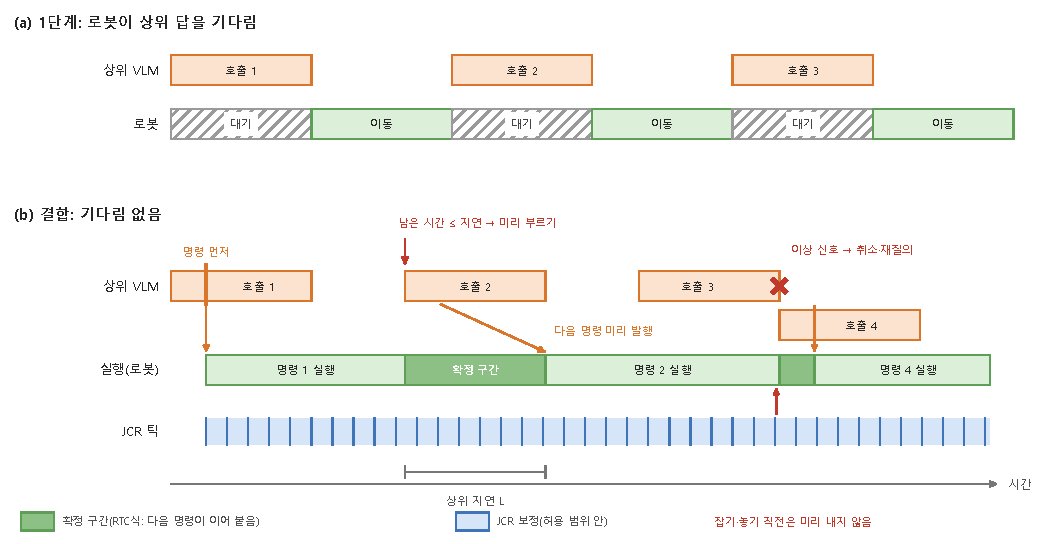
\includegraphics[width=\linewidth]{figures/f4_timeline.pdf}
\caption{\textbf{결합 시간축(개념도, 시간 눈금 없음).} (a) 1단계: 로봇은 상위가 답하는 동안 기다린다. (b) 결합: 재질의는 도착 뒤, 곧 상위가 학습한 장면 그대로다. 상위가 1--3\,s 생각하는 동안 JCR는 끌림을 따라 정렬·잡기·들기 시작을 이어가 로봇이 멈추지 않는다. 이상 신호가 오면 도착 전이라도 취소하고 다시 묻는다. 도착 전 미리 부르기(점선, 선택)는 상위 추가 학습이 필요한 나중 확장이다.}
\label{fig:timeline}
\end{figure*}

명령 먼저 출력과 도착 뒤 재질의 두 가지를 함께 쓴다(\cref{fig:timeline}).
\begin{enumerate}
  \item \textbf{명령 먼저 출력:} 상위 답의 맨 앞에 명령을 두고, 명령 부분이 생성되는 즉시 어댑터를 거쳐 실행한다. 고정 프롬프트는 캐시한다. 호출당 첫 명령까지의 시간을 잰다.
  \item \textbf{도착 뒤 재질의, 생각하는 동안 JCR가 이어감:} 상위를 다시 부르는 시점은 도착 뒤로 고정한다 — 상위가 학습 때 본 장면(1단계의 `도착·검증'과 같은 상황)을 그대로 준다. 호출에 걸리는 1--3\,s(측정한 호출 지연) 동안 로봇을 세워 두지 않고, 어댑터가 JCR에 작은 이어가기 명령을 준다: 잡기 성공 뒤에는 들기 시작 +3\,cm, 놓은 뒤에는 +2\,cm 물러나기다. 예상 밖 접촉·대상 이동 등 이상 신호가 오면 도착 전이라도 취소하고 즉시 다시 묻는다.
\end{enumerate}
평가는 판당 대기 시간, 성공률, 취소율을 함께 보며, 연결 손실이 나빠지지 않아야 채택한다.

\paragraph{(선택) 확장: 도착 전 미리 부르기.} 사건 기준 미리 부르기~\cite{eventtrig2026}와 RTC식 겹치기~\cite{black2025rtc}로 상위가 도착 전에 다음 명령을 미리 내게 할 수 있지만, 이는 상위가 아직 학습하지 않은 입력(도착 예상 표시)과 출력(미리 내도 되나 표지)을 요구해 상위 추가 학습이 필요하다. 지금은 선발행 확률 $p_{\text{pre}} = 0$으로 꺼 두고, 상위 성능을 유지한 채로 결합이 먼저 되는지 본 뒤의 나중 선택지로 둔다(\cref{sec:mesh}).

\subsection{학습: 상위는 동결, JCR만 어댑터 명령으로}
\label{sec:mesh}

\begin{figure*}[t]
\centering
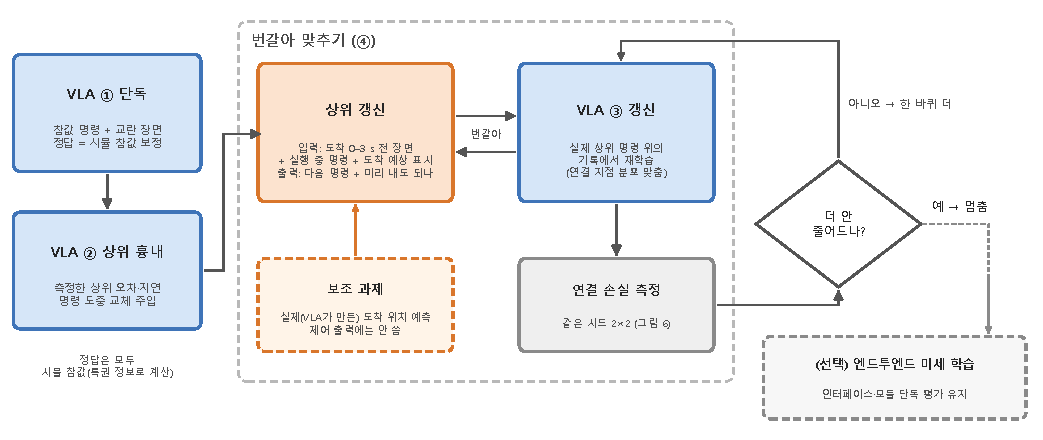
\includegraphics[width=\linewidth]{figures/f5_training.pdf}
\caption{\textbf{결합 학습 루프.} 상위는 지금 학습한 체크포인트로 동결한다. JCR는 단독(①)과 상위 오차 흉내(②)로 시작해, 동결한 상위 + 코드 어댑터를 붙여 돈 실제 기록에서 다시 학습하고(③), 라운드마다 반복 정착한다(④, JCR만 갱신). 매 바퀴 같은 시드 2$\times$2로 연결 손실을 잰다. 더 줄지 않으면 멈춘다. 엔드투엔드 미세 학습과 상위 미리 내기 학습은 그 뒤의 선택지다.}
\label{fig:train}
\end{figure*}

상위 VLM을 건드리지 않는 것이 최우선이므로, 결합 학습은 JCR 쪽에서만 일어난다. 코드 어댑터는 규칙이라 학습이 없다.
\begin{itemize}
  \item \textbf{JCR: 어댑터가 실제로 내는 명령으로.} 시뮬 참값 명령이든 상위 흉내 명령이든, 실제 상위가 낸 명령이든 모두 같은 어댑터(\cref{sec:adapter})를 거친 뒤 JCR에 들어간다 — 상위 흉내 명령도 예외가 아니다(\cref{sec:vla}). 연결 손실은 이 어댑터를 포함한 전체 파이프라인으로 측정한다(\cref{sec:closs}).
  \item \textbf{JCR: 실제 상위 명령 위에서.} 동결한 실제 상위를 붙여 돈 기록에서 참값 보정으로 다시 학습해, 학습 때의 명령 분포와 실행 때의 명령 분포 차이를 없앤다(4단계 중 ③, \cref{sec:vla}).
  \item \textbf{반복 정착.} 라운드마다 실제 상위+어댑터 기록을 다시 모아 JCR만 계속 갱신하고(상위는 그대로), 연결 손실이 더 줄지 않으면 멈춘다(\cref{fig:train}).
  \item \textbf{(선택) 상위 학습이 필요한 확장.} 도착 전 미리 부르기·도착 위치 예측(\cref{sec:timing})은 상위에게 새 입력(도착 예상 표시)과 출력(미리 내도 되나 표지)을 학습시켜야 하므로, 결합이 먼저 되는지 본 뒤의 나중 선택지다.
  \item \textbf{(선택) 엔드투엔드.} 모듈별 학습과 연결 손실 측정이 끝난 뒤, 모은 데이터로 전체를 미세 학습할 수 있다. 이때도 명령 권한 구조(상위 명령 $\rightarrow$ 어댑터 $\rightarrow$ 조이스틱 보정)와 모듈 단독 평가는 유지하고, 전후를 같은 2$\times$2로 비교한다.
\end{itemize}

\subsection{연결 손실}
\label{sec:closs}

\begin{figure*}[t]
\centering
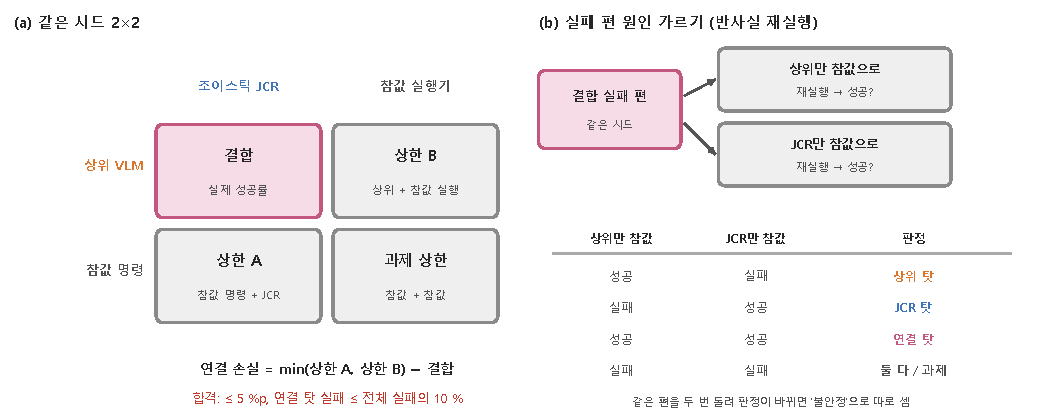
\includegraphics[width=\linewidth]{figures/f6_coupling_loss.pdf}
\caption{\textbf{연결 손실과 원인 분리.} (a) 같은 시드에서 \{상위, 참값 명령\} $\times$ \{JCR, 참값 실행기\} 네 칸을 돌린다. 참값은 시뮬 특권 정보로 계산한 명령·실행이다. (b) 결합 실패 편은 한쪽만 참값으로 바꿔 다시 돌려 원인을 가른다. 판정이 바뀌는 편은 `불안정'으로 따로 센다.}
\label{fig:closs}
\end{figure*}

같은 시드에서 네 칸의 성공률을 잰다(\cref{fig:closs}a). $S_{\text{결합}}$은 상위+JCR, $S_A$는 참값 명령+JCR, $S_B$는 상위+참값 실행기, $S_{\text{과제}}$는 참값+참값이다.
\begin{equation}
  \mathrm{CL} \;=\; \min(S_A,\ S_B) \;-\; S_{\text{결합}}.
\end{equation}
네 칸 모두 같은 코드 어댑터를 거친다 — 참값 명령도 어댑터가 JCR 명령(목적지·마스크·단계·허용·끌림 세기)으로 바꾼 뒤 준다. $S_A$와 $S_B$는 각 모듈이 완벽한 짝을 만났을 때의 상한이므로, 둘 중 낮은 쪽보다 결합이 더 낮은 만큼이 연결에서 샌 성능이다. 결합 실패 편은 한쪽만 참값으로 바꿔 재실행한다. 상위만 바꿔 성공하면 상위 탓, JCR만 바꿔 성공하면 JCR 탓, 어느 쪽을 바꿔도 성공하면 각자는 참값 짝과 되는데 둘이 함께 실패한 것이므로 연결 탓, 둘 다 실패하면 둘 다 또는 과제 탓으로 적는다(\cref{fig:closs}b). 같은 편을 두 번 돌려 판정이 바뀌면 `불안정'으로 따로 센다. 시뮬 물리는 매 편 시작에서 장면을 다시 만들어 같은 시드가 같은 궤적을 재생한다.

\paragraph{합격 기준.} $\mathrm{CL} \le 5$\,\%p, 그리고 연결 탓 실패 $\le$ 전체 실패의 10\,\%. 두 조건을 모두 넘어야 H-C를 지지한다고 본다.

\section{데이터}
\label{sec:data}

\begin{figure*}[t]
\centering
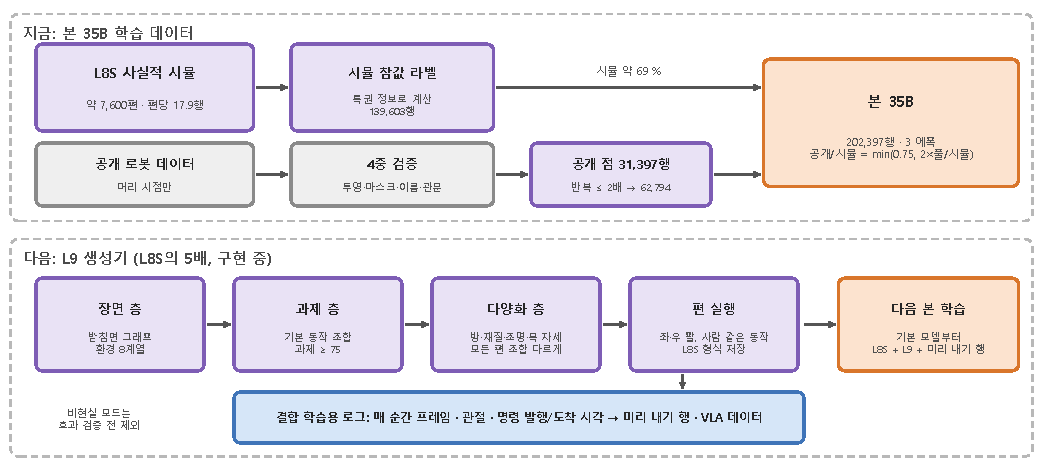
\includegraphics[width=\linewidth]{figures/f7_data.pdf}
\caption{\textbf{데이터 파이프라인.} 위: 본 35B의 데이터. L8S의 시뮬 참값 라벨과, 4중 검증을 통과한 공개 로봇 데이터의 점 라벨을 섞는다. 아래: 다음 데이터 L9. 장면·과제·다양화 층만 새로 만들고 편 실행·저장은 L8S 형식을 쓴다. 결합 학습용 로그(프레임·관절·명령 발행/도착 시각)도 함께 남긴다.}
\label{fig:data}
\end{figure*}

\paragraph{L8S (사실적 시뮬).} 실물 3D 물체, 방 배경, 조명·HDR·재질 무작위화, 센서 현실감(노출·잡음·흐림)을 쓴 시뮬 데이터다. 편의 약 15\,\%에서 목 각도를 흔든다(좌우 ±15$^\circ$, 상하 ±10$^\circ$). 과제는 상자·바구니·통에 넣기, 선반 칸에 놓기, 쌓기, 관계 놓기, 고리 꽂기 등 30종이 넘는 기물 상호작용이다. 관절 한 걸음이 0.04\,rad를 넘는 편은 만들지 않고, 관절 기록이 없어 튐을 검증할 수 없는 서랍 과제는 뺐다. 약 7,600편, 편당 평균 17.9행(조종 11.0 + 보조 6.9), 학습 139,603행(고리 꽂기 1,216행 포함)이다.

\paragraph{공개 점.} 남의 로봇 데이터는 행동 라벨로 쓰지 않고 머리(1인칭) 시점 영상 위의 점 라벨로 바꾼다. 좌표계 정보가 없는 원천은 로봇 몸 실루엣을 영상 속 팔 마스크에 맞춰 카메라를 만들고, 재투영 오차 관문(\tentative{$\le$5\,px})을 넘은 편만 쓴다. 투영 오차, 분할 마스크, 물체 이름 일치, 관문의 4중 검증을 통과한 행만 남긴다. 채택 풀은 32,365행이고, 검증 3\,\%를 뺀 31,397행을 쓴다. 본 학습에서는 반복 상한 2배에 걸려 62,794행(공개/시뮬 약 \tentative{0.45})이다. 3인칭(RH20T, DROID 등)·어안 영상, 관문 경계 행, 라이선스가 NC·ND인 데이터는 쓰지 않는다.

\paragraph{L9 (다음).} L8S의 5배 양·과제·다양성을 목표로 하는 생성기다(설계 확정, 구현 중). 성공 편 $\ge$ 38,000, 과제 정의 $\ge$ 75, 물체 에셋 $\ge$ 6,000, 가구 $\ge$ 1,400, 방 $\ge$ 190, 재질 $\ge$ 650, HDRI $\ge$ 140, 조명 계열 $\ge$ 10이고, 목 자세는 모든 편에서 흔든다. 환경은 8계열(선반장, 식탁, 낮은 탁자, 주방, 현관, 사무실 책상, 가게 진열대, 작업대)이다. 팔은 좌·우를 모두 쓰고(각 40--60\,\%), 두 팔 협업(15--20\,\%)은 2단계로 둔다. 모든 편의 환경 조합 해시가 달라야 하고, 머리 영상 SigLIP 임베딩에서 거의 같은 장면의 비율이 L8S보다 낮아야 한다. 참값 궤적은 사람 같은 동작(두 구간 최소 저크 뻗기, 물체 크기에 맞춘 그리퍼 벌림, 자세 선호, 편마다 다른 조작 성향)을 따른다. 비현실 겉모습 모드는 만들되 효과를 확인하기 전에는 학습에 넣지 않는다. 다른 로봇의 데이터는 로봇 몸에 머리 카메라가 있을 때만 쓴다. 결합 학습을 위해 매 순간의 프레임, 관절값, 명령 발행·도착 시각을 로그에 남긴다.

\section{평가 체계}
\label{sec:eval}

\begin{figure*}[t]
\centering
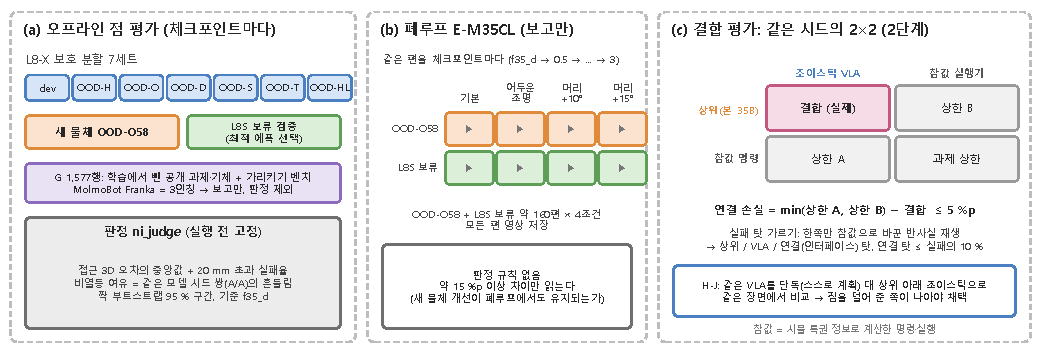
\includegraphics[width=\linewidth]{figures/eval_protocol.pdf}
\caption{\textbf{평가 체계.} (a) 체크포인트마다 오프라인 점 평가. (b) 폐루프 E-M35CL(보고 전용). (c) 결합 평가: 같은 시드 2$\times$2와 원인 분리, H-J 비교. 참값은 시뮬 특권 정보로 계산한 명령·실행이다.}
\label{fig:eval}
\end{figure*}

\paragraph{오프라인 점.} L8-X 보호 분할 7세트(dev\_x, 본 적 없는 탁자 높이 OOD-H, 리프트 범위의 보류 높이 OOD-H-lift, 새 물체 범주 OOD-O, 보류 방해물·재질·조명 OOD-D, 보류 조합 OOD-T, 보류 가구 OOD-S), 학습에 한 번도 나오지 않은 실물 13종의 새 물체 세트 OOD-O58(\tentative{58}편), L8S 보류 검증, 일반 평가 G(학습에서 뺀 공개 과제·기체와 공개 가리키기 벤치, 1,577행)를 쓴다(\cref{fig:eval}a). G의 MolmoBot Franka 세트는 전부 3인칭·어안이라 보고만 하고 판정에서 뺀다. 지표는 접근 목표 3D 오차의 중앙값과 20\,mm 초과 실패율이다. 비열등 여유는 같은 모델의 두 시드(A/A) 흔들림으로 정하고, 같은 스냅숏 짝 부트스트랩 95\,\% 구간으로 판정한다.

\paragraph{폐루프.} 새 물체 OOD-O58과 L8S 보류 편을 기본, 어두운 조명, 머리 기울기 +10$^\circ$·팬 +15$^\circ$ 변형으로 체크포인트마다 돌린다(E-M35CL, \cref{fig:eval}b). 편당 한 번이라 약 15\,\%p 이상의 차이만 읽는 보고 전용이며, 모든 편의 머리·손목 영상을 저장한다.

\paragraph{결합.} 같은 시드 2$\times$2로 연결 손실과 원인 비율을 재고(\cref{sec:closs}), 같은 VLA를 단독 모드와 조이스틱 모드로 돌려 H-J를 비교하며, 판당 대기 시간·취소율을 함께 적는다(\cref{fig:eval}c). 세트는 새 물체, L8S 보류, L9 보류다.

\paragraph{절차.} 모든 실험은 ``이 결과로 바꾸는 결정''과 판정 규칙을 실행 전에 사전 등록한다. 판정 규칙을 바꾸면 등록 문서에 변경으로 남기고, 관문을 넘기는 결정은 기록과 함께 사람이 한다.

\section{지금까지의 근거}
\label{sec:evidence}

\begin{figure*}[t]
\centering
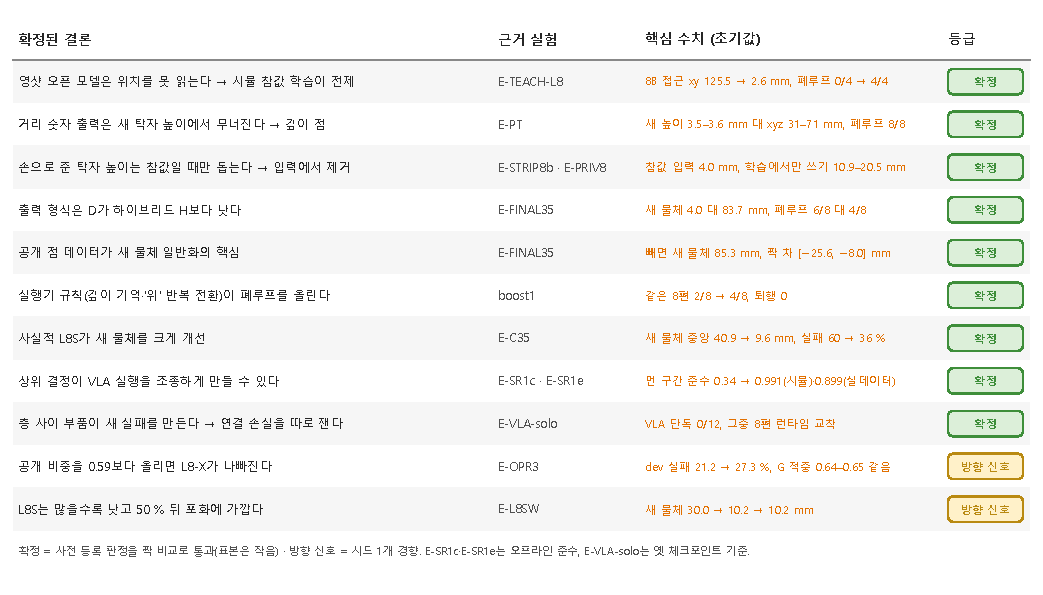
\includegraphics[width=\linewidth]{figures/f8_conclusions.pdf}
\caption{\textbf{확정된 결론 지도.} 결론마다 근거 실험, 핵심 수치(모두 \tentative{초기값}), 신뢰 등급을 적었다. 확정 = 사전 등록 판정을 짝 비교로 통과(표본은 작다). 방향 신호 = 시드 하나의 경향. E-SR1c·E-SR1e는 오프라인 준수이고, E-VLA-solo는 앞선 두 층 구현의 체크포인트 기준이다.}
\label{fig:concl}
\end{figure*}

모든 실험은 판정 규칙을 실행 전에 고정했다. 표본이 작고 시드가 하나인 경우가 많으므로 수치는 모두 초기값이다. \cref{fig:concl}은 지금 확정된 결론을 한눈에 모은 것이다.

\paragraph{상위는 학습해야 조종할 수 있다 (H-L).} 영샷 Qwen3-VL-8B는 접근 목표 xy 오차 중앙이 \tentative{125.5\,mm}였고, 시뮬 참값 라벨로 LoRA 학습하자 \tentative{2.6\,mm}, 폐루프 \tentative{0/4 $\rightarrow$ 4/4}가 되었다(E-TEACH-L8). 영샷 8B에게 점을 찍게 해도 점이 \tentative{55--95\,px} 빗나갔으므로 점 형식도 학습이 전제다.

\paragraph{거리는 깊이 점이 알려 준다.} 같은 편을 출력 형식만 바꿔 비교하자, 깊이 점만 본 적 없는 탁자 높이에서 \tentative{3.5--3.6\,mm}를 유지했고(깊이 없는 xyz \tentative{31--71\,mm}) 폐루프 \tentative{8/8}이었다(E-PT). 참 탁자 높이를 입력한 판만 새 높이에 맞았고(\tentative{4.0\,mm}), 학습에서만 쓰는 세 방법은 \tentative{10.9--20.5\,mm}로 채택 기준을 넘지 못했다(E-STRIP8b, E-PRIV8).

\paragraph{D와 공개 점.} 35B를 D와 하이브리드 H로 학습해 비교하자 새 물체에서 D \tentative{4.0} 대 H \tentative{83.7\,mm}, 폐루프 \tentative{6/8} 대 \tentative{4/8}이었고 나머지 다섯 세트는 같았다(E-FINAL35, 판마다 시드 하나). 공개 점만 뺀 D는 새 물체 \tentative{85.3\,mm}, 폐루프 \tentative{2/8}이었다(짝 차 \tentative{[$-$25.6, $-$8.0]\,mm}). 재학습 없는 실행기 규칙은 같은 8편에서 \tentative{2/8 $\rightarrow$ 4/8}, 퇴행 0이었다(boost1). 이 35B D(f35\_d)가 본 학습의 비교 기준이다.


\paragraph{데이터 구성.} 사실적 L8S로 만든 확인판(E-C35)은 새 물체 OOD-O58 오차 중앙을 \tentative{40.9 $\rightarrow$ 9.6\,mm}, 실패율을 \tentative{60 $\rightarrow$ 36\,\%}로 줄였다. 반면 L8-X dev 실패(\tentative{16.8 $\rightarrow$ 27.5\,\%})와 OOD-H(\tentative{17.3 $\rightarrow$ 22.8\,\%})는 나빠졌다. 공개 비중을 0.59보다 올리면 L8-X가 나빠지고 G는 나아지지 않았다(E-OPR3, \cref{fig:evidence}c). L8S는 많을수록 나았고 50\,\% 뒤로는 포화에 가까웠다(E-L8SW, \cref{fig:evidence}b). 두 결과 모두 시드 하나의 방향 신호다.

\paragraph{본 35B.} 1 에폭에서 새 물체 오차 중앙·실패율은 \tentative{9.5\,mm / 34.8\,\%}로 f35\_d(\tentative{40.9\,mm / 60\,\%})보다 크게 나았다. L8-X dev \tentative{4.5\,mm / 18.9\,\%}(f35\_d \tentative{4.4 / 16.8}), OOD-H \tentative{4.0 / 17.3}(같음), OOD-O \tentative{4.1 / 37.4}(\tentative{4.1 / 40.8}), 일반 평가 G 적중 \tentative{0.742}(\tentative{0.713}), L8S 보류 \tentative{5.5\,mm / 23.7\,\%}였다. 확인판에서 벌어졌던 옛 도메인 차이는 학습이 진행될수록 줄어(\cref{fig:evidence}d), 그 손해가 도메인보다 양 때문이라는 해석과 맞는다. 최종 판정은 사전 등록한 최적 에폭에서 낸다.

\paragraph{결합 쪽 근거.} 상위 결정 토큰만 바꿔서는 VLA의 행동 청크가 거의 움직이지 않았다(강제 방향 준수 \tentative{0.34}, 우연 약 0.33, E-SR0). 물체에서 먼 구간의 반사실 분기를 흐름 정합 학습에 섞자 준수가 시뮬 \tentative{0.991}(E-SR1c), 실데이터 \tentative{0.899}(E-SR1e, 두 시드)로 올랐고 접촉 근처 능력은 비열등이었다. 오프라인 준수이며 폐루프 확인은 아니다. 앞선 두 층 구현에서 VLA 단독은 모든 조건에서 \tentative{0/12}였고(같은 장면 스크립트 기준선 \tentative{12/12}), 그중 \tentative{8}편은 모델이 아니라 층 사이 런타임의 멈춤 고리였다(E-VLA-solo). 층 사이의 부품이 새 실패를 만든다는 이 결과가, 연결 손실을 따로 재는 이유다.

\paragraph{JCR를 따로 학습해야 한다 (E-CJ1).} 상위 없이 시뮬 참값 명령을 주고, 같은 시드(머그$\rightarrow$쟁반, 20 배치 $\times$ 기본·무작위화 = 팔당 40편)에서 세 팔을 비교했다. 스크립트 실행기(OX)는 \tentative{40/40}, 앞의 오프라인 준수 \tentative{0.991} 체크포인트를 조이스틱으로 쓴 OV는 \tentative{1/40}, 같은 모델의 단독 모드(V0)는 \tentative{0/40}이었다. 등록 규칙상 이 모델은 조이스틱으로도 과제를 못 하는 바닥(VLA\_FLOOR)이므로 2$\times$2보다 JCR 학습이 먼저다. OV의 결정 스텝 약 10,000개를 나눠 보면 원인은 네 가지다.
\begin{itemize}
  \item \textbf{분포 이동:} 폐루프 xy 준수는 \tentative{0.41}(목표에서 먼 구간 \tentative{0.47})로, 학습 분포 안 상태에서 잰 오프라인 \tentative{0.991}과 달랐다. 좌표계 오류의 흔적(일정한 회전)은 없었다.
  \item \textbf{근접 구간을 배운 적 없음:} 반사실 분기가 먼 구간에만 있었다. 목표 2\,cm 안 스텝의 \tentative{77\,\%}가 오히려 멀어졌고(준수 \tentative{0.33}), 손은 대상 위 3--9\,cm에서 맴돌았다.
  \item \textbf{거친 조이스틱:} 8방향·5단 크기·축별 1\,cm 사각지대라 방향 양자화 오차가 90분위 \tentative{35$^\circ$}였고, 8\,mm 수렴이 구조적으로 어려웠다.
  \item \textbf{청크 이음 계단:} 청크 첫 행과 현재 관절의 차가 중앙 \tentative{0.065\,rad}로, 청크의 \tentative{87.5\,\%}가 0.04\,rad 한도에 잘렸다. 또 그리퍼 시점은 접촉이 아니라 단계 문장을 따랐다.
\end{itemize}
지연은 원인이 아니었다(모델 호출 동안 시뮬 시간이 멈춤). 네 원인이 JCR 설계의 네 선택, 곧 자기 롤아웃 재라벨, 근접 분기, 연속 조이스틱, 명령 기준 TCP 변위 청크와 단계 문장 제거로 이어진다(\cref{sec:vla}).

\section{남은 질문}
\label{sec:questions}
\begin{itemize}
  \item 상위 판단(진행 평가, 실패 감지)의 정확도는 얼마인가? 이를 재는 평가 세트와 지표부터 만들어야 한다.
  \item 도착 전 다음 명령은 몇 초 전까지 맞출 수 있는가($\Delta=0$--3\,s 정답률 곡선)?
  \item 짐을 덜어 준 JCR가 실제로 같은 JCR 단독보다 나은가(H-J)?
  \item 연결 손실을 5\,\%p 안으로, 연결 탓 실패를 10\,\% 안으로 줄일 수 있는가(H-C)? 원인 분리 실험(E-CJ3)은 등록 전이다.
  \item 최종 JCR의 기반 모델과 보정 주기(Hz)는 무엇이 맞는가?
  \item 공개/시뮬 최적 비율, 손목 카메라의 기여, LoRA로 충분한지는 뒤로 미룬 문제다.
\end{itemize}

{
    \small
    \bibliographystyle{ieeenat_fullname}
    \bibliography{main}
}
\end{document}
